\subsection{Ví dụ tiêu biểu}
%%--------frame 1-------
\begin{frame}{Ví dụ tiêu biểu}
    \begin{mypro*}{}
        Theo khảo sát của sinh viên đối với ba quán cafe $A, B, C$, ta biết rằng ban đầu, hai quán $A, B$ chưa mở nên $100\%$ khách đều đến $C$ và:
    \begin{itemize}
        \item[\bullet] Trong những sinh viên đến quán $A$, sẽ có $20\%$ người tiếp tục đến $A$, có $60\%$ người sang $B$ và có $20\%$ người sang $C$.
        \item[\bullet] Trong những sinh viên đến quán $B$, sẽ có $40\%$ người tiếp tục đến $B$, có $10\%$ người sang $A$ và có $50\%$ người sang $C$.
        \item[\bullet] Trong những sinh viên đến quán $C$, sẽ có $10\%$ người tiếp tục đến $C$, có $70\%$ người sang $A$ và có $20\%$ người sang $B$.
    \end{itemize}

    \begin{itemize}
        \item[(a)] Hãy tìm xem tỉ lệ phần trăm người đến quán $A$, $B$, $C$ sau 3 tuần.
        \item[(b)] Hãy tìm xem tỉ lệ sinh viên đến quán $B$ ở tuần thứ 5 biết rằng tuần thứ 2 ở quán $C$ và tuần thứ 3 ở quán $A$.
        \item[(c)] Hãy tìm xem tỉ lệ sinh viên đến quán $B$ ở tuần thứ 2 và đến quán $A$ ở tuần thứ 4 biết rằng đến quán $B$ ở tuần thứ 3.
    \end{itemize}
    \end{mypro*}
\end{frame}
%%--------frame 2-------
\begin{frame}{Ví dụ tiêu biểu}
    Thời gian chúng ta xét sẽ là tuần. Tiếp theo ta có không gian trạng thái $S = \{A, B, C \}$. Đặt $X_t$ là biến ngẫu nhiên đại diện cho quán cafe mà sinh viên đến ở tuần thứ $t$ và có phân phối ban đầu $\pi_0$ là
$$
\pi_0 = \begin{bmatrix}
\P(X_0 = A) & \P(X_0 = B) & \P(X_0 = C) 
\end{bmatrix} = \begin{bmatrix}
    0 & 0 & 1
\end{bmatrix}
$$

\noindent Dựa theo đề bài ta có ma trận chuyển tiếp $\mathbf{P}$ là:
$$
\mathbf{P} = \begin{bmatrix}
    P_{AA} & P_{AB} & P_{AC} \\
    P_{BA} & P_{BB} & P_{BC} \\
    P_{CA} & P_{CB} & P_{CC}
\end{bmatrix} = \begin{bmatrix}
    0.2 & 0.6 & 0.2 \\
    0.1 & 0.4 & 0.5 \\
    0.7 & 0.2 & 0.1
\end{bmatrix}
$$

\noindent Ta biểu diễn chuỗi Markov trên thành đồ thị như dưới đây:
\begin{figure}[H]
    \centering
    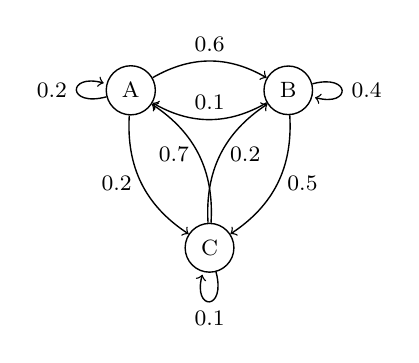
\begin{tikzpicture}[-> , line width=0.5 pt ,node distance =1 cm]
        \tikzstyle{every node}=[font=\footnotesize]
        
        \node[circle, draw] (A) at (0,0) {A};
        \node[circle, draw] (B) at (2,0) {B};
        \node[circle, draw] (C) at (1, -2) {C};
        
        \path (A) edge [bend left] node [above] {$0.6$} (B);
        \path (A) edge [loop left] node{$0.2$} (A);
        \path (A) edge [bend right] node [left] {$0.2$} (C);

        \path (B) edge [bend left] node [above] {$0.1$} (A);
        \path (B) edge [loop right] node{$0.4$} (B);
        \path (B) edge [bend left] node [right] {$0.5$} (C);

        \path (C) edge [bend right] node [left] {$0.7$} (A);
        \path (C) edge [bend left] node [right] {$0.2$} (B);
        \path (C) edge [loop below] node{$0.1$} (C);
        
    \end{tikzpicture}
    \caption{Đồ thị $G$ biểu diễn của chuỗi Markov của bài toán} 
    \label{fig:graphprob}
\end{figure}
\end{frame}
%%--------frame 3-------
\begin{frame}{Ví dụ tiêu biểu}
\noindent Tính toán luỹ thừa 2 và 3 của ma trận chuyển tiếp $\mathbf{P}$, ta được:
$$
\mathbf{P}^2 = \begin{bmatrix}
    0.24 & 0.4 & 0.36 \\
    0.41 & 0.32 & 0.27 \\
    0.23 & 0.52 & 0.25
\end{bmatrix} \hspace{10pt} \text{và} \hspace{10pt}
\mathbf{P}^3 = \begin{bmatrix}
    0.34 & 0.376 & 0.284 \\
    0.303 & 0.428 & 0.269 \\
    0.273 & 0.396 & 0.331 
\end{bmatrix}
$$

\begin{itemize}
    \item[(a)] Ta có tỉ lệ sinh viên đến quán $A, B, C$ ở tuần thứ 3 chính là $\pi_3$, do đó:
    $$
    \pi_3 = \pi_0 \mathbf{P}^3 = \begin{bmatrix}
        0.273 & 0.396 & 0.331
    \end{bmatrix}
    $$

    \item[(b)] Tỉ lệ sinh viên đến quán $B$ ở tuần thứ 5 biết rằng tuần thứ 2 ở quán $C$ và tuần thứ $3$ ở quán $A$ chính là:
    $$
    \begin{aligned}
    \P(X_5 = B \mid X_2 = C, X_3 = A) &= \P(X_5 = B \mid X_3 = A) \\
    &= \P(X_2 = B \mid X_0 = A) = P^2_{AB} = 0.4
    \end{aligned}
    $$

    \item[(c)] Tỉ lệ sinh viên đến quán $B$ ở tuần thứ 2 và đến quán $A$ ở tuần thứ 4 biết rằng đến quán $B$ ở tuần thứ 3 chính là:
    $$
    \begin{aligned}
    \P(X_2 = B, X_4 = A \mid X_3 = B) &= \P(X_4 = A \mid X_3 = B) \P(X_2 = B \mid X_3 = B) \\
    &= \P(X_1 = A \mid X_0 = B) \dfrac{\P(X_3 = B \mid X_2 = B) \P(X_2 = B)}{\P(X_3 = B)} \\
    &= P_{BA}P_{BB} \dfrac{\pi_2(B)}{\pi_3(B)} \approx 0.052525 
    \end{aligned}
    $$
\end{itemize}
\end{frame}
%%--------frame 4-------
\begin{frame}{Ví dụ tiêu biểu}
    \begin{mypro*}{}
Một khảo sát được thực hiện trên 100 người dùng điện thoại. Ban đầu có 60 người dùng điện thoại sử dụng hệ điều hành Android, 40 người dùng điện thoại sử dụng hệ điều hành IOS. Sau mỗi quý, sẽ có 12 người chuyển từ Android sang IOS, 4 người chuyển từ IOS sang Android. Hãy tìm xem sau 50 quý thì tỉ lệ người dùng ở hai hệ điều hành sẽ như nào, ngoài ra sau 100 quý hay 200 quý hay 500 quý thì có thay đổi gì không ?
    \end{mypro*}
\begin{mysol*}{}
    Thời gian chúng ta xét sẽ là quý. Tiếp theo ta có không gian trạng thái $S = \{A, I\}$ với $A$ viết tắt cho Android và $I$ cho IOS. Đặt $X_t$ là biến ngẫu nhiên cho hệ điều hành mà người dùng sử dụng ở quý thứ $t$ và có phân phối ban đầu $\pi_0$ là:
$$
\pi_0 = \begin{bmatrix}
    \P(X_0 = A) & \P(X_0 = I)
\end{bmatrix} = \begin{bmatrix}
    0.6 & 0.4
\end{bmatrix}
$$

\noindent Dựa theo đề bài ta có ma trận chuyển tiếp $\mathbf{P}$ là:
$$
\mathbf{P} = \begin{bmatrix}
    P_{AA} & P_{AI} \\
    P_{IA} & P_{II} \\
\end{bmatrix} = \begin{bmatrix}
    0.8 & 0.2 \\
    0.1 & 0.9 
\end{bmatrix}
$$
\end{mysol*}
\end{frame}
%%--------frame 5-------
\begin{frame}{Ví dụ tiêu biểu}
\begin{mysol*}{(tt)}
    \noindent Khi đó tỉ lệ người dùng sau 50 quý hay nói cách khác là phân phối tại $t = 50$ là:
$$
\pi_{50} = \pi_0 \mathbf{P}^{50} = 
\begin{bmatrix}
    0.333 & 0.6667
\end{bmatrix}
$$

\noindent Tiếp theo tỉ lệ người dùng sau 100 quý sẽ là:
$$
\pi_{100} = \pi_0 \mathbf{P}^{100} = \begin{bmatrix}
   0.33333333 & 0.66666667 
\end{bmatrix}
$$

\noindent Tỉ lệ người dùng sau 500 quý sẽ là:
$$
\pi_{500} = \pi_0 \mathbf{P}^{500} = \begin{bmatrix}
    0.33333333 & 0.66666667
\end{bmatrix}
$$
\end{mysol*}
\noindent Ta có thể thấy, kể từ 100 quý trở về sau, phân phối sẽ không thay đổi nữa. Điều này làm ta có thể nghĩ đến việc phân phối của chuỗi Markov có ``giới hạn'' và phân phối giới hạn đó được gọi là \textbf{phân phối bất động} (stationary distribution), kí hiệu là $\pi$:
$$
\pi_n = \pi_0 \mathbf{P^n} \xrightarrow{n \to \infty} \pi
$$

\noindent Trong trường hợp của bài toán này phân phối bất động chính là:
$$
\pi = \begin{bmatrix}
    \dfrac{1}{3} && \dfrac{2}{3}
\end{bmatrix}
$$
\end{frame}
%%--------frame 6-------
